\documentclass{beamer}

\usetheme{focus}
\usepackage{booktabs}
\usepackage{minted}
\usepackage{caption}
% \usepackage{subcaption}
% \usepackage{subfig}

\usepackage[unicode]{hyperref}
\hypersetup{colorlinks,citecolor=green,filecolor=green,linkcolor=blue,urlcolor=blue}


\title{Razvoj rekurentne neuronske mreže i primena na analizi \\ vremenskih serija}
\subtitle{\small{Seminarski rad u okviru kursa\\Računarska inteligencija}}
\author{\small{Kristina Pantelić, 91/2016, mi16091@matf.bg.ac.rs \\Nevena Mesar, 107/2015, mi15107@matf.bg.ac.rs }}

\institute{Matematički fakultet}
\date{20.6.2020.}
\begin{document}

%--------------------------------------------------------
\begin{frame}
    \maketitle
\end{frame}

%--------------------------------------------------------
\begin{frame}{Uvod}
    \begin{itemize}
        \item Tradicionalna neuronska mreža
            \begin{itemize}
             \item ulazi i izlazi nezavisni jedni od drugih
            \end{itemize} 
        \item Rekurentna neuronska mreža
             \begin{itemize}
             \item svojstvo pamćenja naučenog znanja iz prethodnih trening instanci
             \item omogućava predikciju u oblasti vremenskih serija
              \end{itemize}
        \item Jordanova rekurentna neuronska mreža (eng. \textit{Jordan SRNN})
            \begin{itemize}
             \item kopija izlaznog sloja se sprovodi na ulaz
            \end{itemize}
    \end{itemize}
\end{frame}

%--------------------------------------------------------
\begin{frame}{Jordan SRNN}
    \begin{figure}
        \centering
        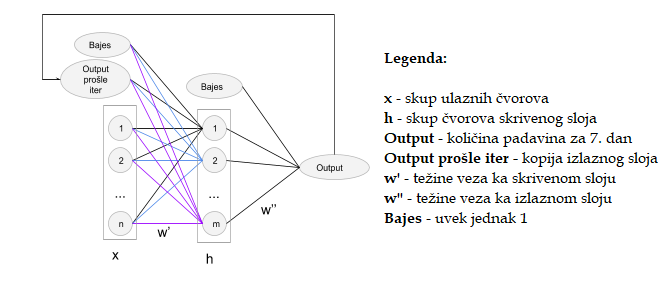
\includegraphics[scale=0.6]{net.png}
        \caption{Jordanova SRNN sa jednim skrivenim slojem}
    \end{figure}
\end{frame}

%--------------------------------------------------------
\begin{frame}{Model RNN-a}
    \begin{itemize}
    \item \textbf{Aktivaciona funkcija} skrivenog i izlaznog sloja:
    $$f(x)=(1+e^{-x})^{-1}$$
    \item Greška izlaznog sloja neurona k: \\
    $$E_k = \frac{1}{2}(y_k - o_k)^2$$
    \item Pri ažuriranju vrednosti $w{''}_{jk}$, važi $w{''}_{jk}=w{''}_{jk}+\Delta{}w{''}_jk$, gde je
$$\Delta{} w{''}_{jk}=- \eta{}\frac{\partial{}E_k}{\partial{}w{''}_{jk}}+\alpha{}\Delta{}w{''}_{jk}$$
    $\eta{}$ uticaj parcijalnog izvoda greške $E_k$ po $w{''}_{jk}$ \\
    $\alpha{}$ uticaj prethodne vrednosti $\Delta{}w{''}_{jk}$
    \end{itemize}
\end{frame}

%--------------------------------------------------------
\begin{frame}{Algoritam}
    \begin{enumerate}
  \item Ulazni podaci ($x^{(l)}_1$, $x^{(l)}_2$,..., $x^{(l)}_{n+p}$) i ($y_1$, $y_2$,..., $y_p$),\\
  $x^{(l)}_0=1, {}\forall{l}$ iz skupa podataka
  \item Init $\eta{}$, $\alpha{}$ i kriterijum zaustavljanja\\
  Init $w'_{ij}$ i $w{''}_{jk}$ i $\Delta{}w'_{ij}=\Delta{}w{''}_{jk}=0$
  \item Novi par ulaznog i izlaznog vektora
  \item Odrediti $u'_j$ i $h_j$. Postaviti $h^{(l)}_0=1, {}\forall{l}$ iz skupa podataka
  \item Odrediti $u{''}_k$ i $o_k$. Ukoliko je ispunjen kriterijum zaustavljanja, prekinuti izvršavanje.
  \item Odrediti $\Delta{}w{''}_{jk}$ i ažurirati vrednosti $w{''}_{jk}$.
  \item Odrediti $\Delta{}w{'}_{ij}$ i ažurirati vrednosti $w{'}_{ij}$.
  \item Preći na korak 3.
\end{enumerate}
\end{frame}

%--------------------------------------------------------

% ============ IMPLEMENTACIJA ALGORITMA =================
% \section{Implementacija algoritma}
%--------------------------------------------------------
\begin{frame}{Implementacija algoritma}
    \begin{columns}
		\column{0.6\textwidth}
        \begin{block}{Potrebne biblioteke}
            \begin{itemize}
                \item \texttt{numpy}  -- 
                zeros, array, append, concatenate, multiply, vstack, matrix, around, random
                \item \texttt{pandas} -- DataFrame, Series, read\_csv, errors, concat
                \item \texttt{sklearn} 
                    \begin{itemize}
                        \item metrics -- mean\_absolute\_error, mean\_squared\_error
                        \item model\_selection -- train\_test\_split
                        \item preprocessing -- MinMaxScaler
                    \end{itemize}
                \item \texttt{matplotlib} -- pyplot
            \end{itemize}
        \end{block}
        \column{0.4\textwidth}
        \begin{block}{Izvor podataka}
            \small{
            Basel, Švajcarska\\
            31.12.1990. do 31.12.2019}
            \begin{center}
                \href{https://www.meteoblue.com/en/weather/archive/export/basel_switzerland_2661604}{
\includegraphics[scale=0.3]{presentation/1_meteoblue.jpg}}
            \end{center}
        \end{block}
    \end{columns}
\end{frame}

%--------------------------------------------------------
\begin{frame}{Implementacija algoritma}
    \small{
    \begin{columns}
    \column{0.5\textwidth}
    \begin{block}{Predprocesiranje}
        \begin{itemize}
            \item \texttt{test} : \texttt{train} = 3 : 7 \\ test -- 3398, train -- 7928
            \item \texttt{sklearn.model\_selection} -- \texttt{test\_train\_split}
            \item \texttt{MinMaxScaler} -- [0.1, 0.9]
            \item precipitation \\[0, 100] $\rightarrow$  [0.1, 0.9]
        \end{itemize}
    \end{block}
    \column{0.5\textwidth}
    \begin{block}{Inicijalizacija}
        \begin{itemize}
            \item Broj dana za predikciju: \texttt{N}
            \item Ulazni čvorovi:\\\texttt{n = N * n\_attrs + 1}
            \item Patern: 6 dana + output
            \item Broj paterna:\\\texttt{len(x\_train) - N}
            \item Broj atributa za jedan dan: \texttt{n\_attrs}
            \item Čvorovi skrivenog sloja:\\ \texttt{m = (int)((N * n\_attrs) * 4) + 1}
            \item \texttt{eta = 0.3; alpha = 0.2}
        \end{itemize}
    \end{block}
    \end{columns}
    }
\end{frame}

%--------------------------------------------------------
\begin{frame}[fragile]{Implementacija algoritma -- paterni}
    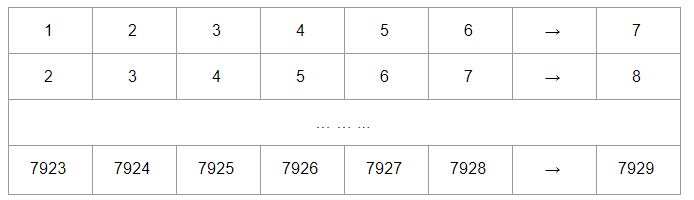
\includegraphics[scale=0.75]{dani.JPG}
    \begin{itemize}
        \item Svaka ćelija je skup atributa za jedan dan
        \item Jedan patern, \texttt{input\_nodes}, predstavlja 6 dana zaredom
        \begin{verbatim}
concatenate((bias, 
            (x_train[day:(day+N)]).reshape(-1), 
            output_arr))
        \end{verbatim}
    \end{itemize}
\end{frame}

%--------------------------------------------------------
\begin{frame}[fragile]{Izračunavanje h1,..., hm čvorova skrivenog sloja}
\begin{columns}
    \column{0.5\textwidth}
    \begin{Verbatim}[fontsize=\small]
# Naivan pristup
h[0] = 1.0
for j in range(1, m+1):
    u = 0
    for i in range(0, n+1):
        u += input_nodes[i] 
            * w_[i][j]
    h[j] = activation_f(u)
    \end{Verbatim}
    \begin{figure}
        \centering
        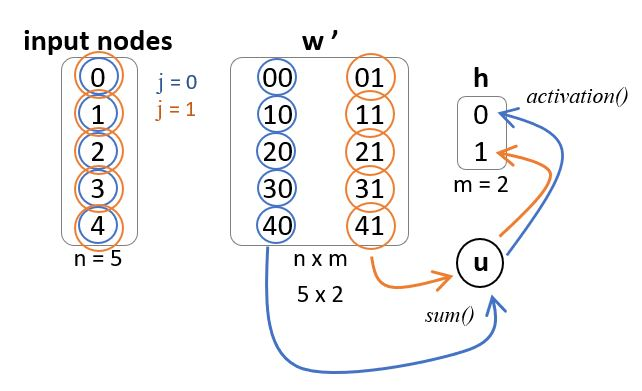
\includegraphics[scale=0.4]{naivno_izracunavanje_w_.JPG}
    \end{figure}
    
    \column{0.5\textwidth}
    \begin{Verbatim}[fontsize=\small]
# Poboljsan pristup
u = []
for i in w_.T:
    u += [activation_f(
            sum(multiply(
                i, 
                input_nodes))
          )]
h = array(u)
h[0] = 1
    \end{Verbatim}
    \begin{figure}
        \centering
        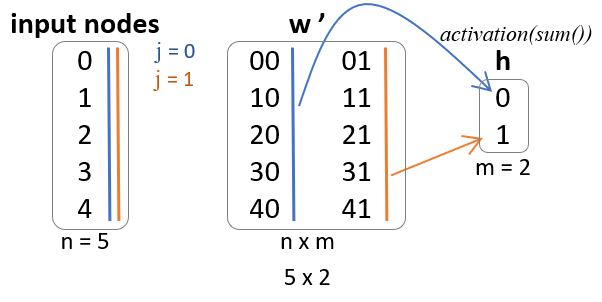
\includegraphics[scale=0.4]{izracunavanje_w_.JPG}
    \end{figure}
    
\end{columns}

\end{frame}


%--------------------------------------------------------
\begin{frame}[fragile]{Izračunavanje o1,...,op i greške}
    \begin{block}{Računanje izlaznog čvora}
    \begin{Verbatim}[fontsize=\small]
# Naivna implementacija
for k in range(1, p+1):
    u = 0
    for j in range(0, m+1):
        u += h[j] * w__[j][k]
    o[day] = activation_f(u)

# Poboljsana implementacija
o[day] = activation_f(sum(multiply(h, w__)))
output_arr = array([o[day]])
    \end{Verbatim}
    \end{block}
    \begin{block}{Računanje greške}
        \texttt{error = (y\_train[day+N] - o[day]) * o[day] * (1.0 - o[day])}
    \end{block}
\end{frame}

%--------------------------------------------------------



%--------------------------------------------------------
\begin{frame}[fragile]{Izračunavanje deltaH(j)}
\begin{verbatim}
# Naivna implementacija
for j in range(1, m+1):
    dh[j] = 0.0
    for k in range(1, p+1):
        dh[j] += w__[j][k] * error
        
# Poboljsana implementacija
dh = w__ * error
\end{verbatim}
\end{frame}

%--------------------------------------------------------
% \begin{frame}[fragile]{Ažuriranje W'(ij) i deltaW'(ij)}
% \begin{verbatim}
% # Bukvalna interpretacija
% for j in range(1,m+1):    
%     for i in range(0,n+1): 
%         dw_[i][j] = eta * input_nodes[i] * h[j] 
%                     * (1 - h[j]) * dh[j] 
%                     + alpha * dw_[i][j] 
%         w_[i][j] += dw_[i][j]
% \end{verbatim}
% \end{frame}


%--------------------------------------------------------
\begin{frame}[fragile]{Ažuriranje W'(ij) i deltaW'(ij)}
\begin{columns}
    \column{0.5\textwidth}
    \begin{Verbatim}[fontsize=\tiny]
# Naivna implementacija
for j in range(1, m+1):
    H = h[j] * (1 - h[j]) * dh[j]
    for i in range(0, n+1):
        dw_[i][j] = eta * input_nodes[i] * H 
                    + alpha * dw_[i][j]
        w_[i][j] += dw_[i][j]
    \end{Verbatim}
    \begin{figure}
        \centering
        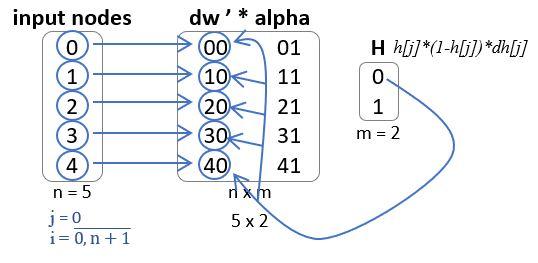
\includegraphics[scale=0.52]{azuriranje_w_.JPG}
    \end{figure}
    
    \column{0.5\textwidth}
    \begin{Verbatim}[fontsize=\tiny]
# Poboljsana implementacija
H = h * (1-h) * dh * eta
dw_ *= alpha
for j in range(0, m):
    dw_.T[j] += (input_nodes * H[j])
w_ += dw_
    \end{Verbatim}
    \begin{figure}
        \centering
        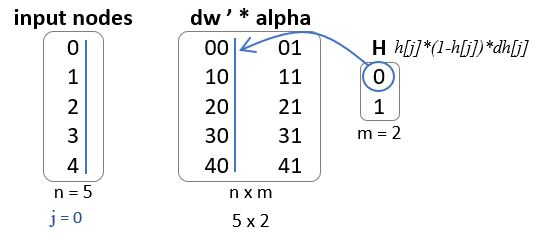
\includegraphics[scale=0.52]{poboljsano_azuriranje_w_.JPG}
    \end{figure}
\end{columns}
\end{frame}

%--------------------------------------------------------
\begin{frame}[fragile]{Ažuriranje W''(jk) i deltaW''(jk)}
    \begin{verbatim}
# Naivna implementacija
for k in range(1, p):
    for j in range(0, m):
        dw__[j][k] = eta * h[j] * error 
                    + alpha * dw__[j][k]
        w__[j][k] += dw__[j][k]
        

# Poboljsana implementacija
dw__ *= alpha
dw__ += (eta * h * error)
w__ += dw__
    \end{verbatim}
\end{frame}

%--------------------------------------------------------
% Reci usmeno
% \begin{frame}{Čuvanje modela i testiranje}
%     \begin{itemize}
%         \item Kroz epohe se beleži najbolji model.
%         \item Moguće je učitati neki od postojećih modela kako bi se uštedelo na vremenu.
%         \item Testiranje se sastoji od primene istih operacija korišćenjem postojećih težinskih matrica nad skupom za test.
%     \end{itemize}
% \end{frame}


% \section{Primeri rezultata}

%========================================================= 1
\begin{frame}{\small{Model \texttt{n = 54, m = 270, alpha = 0.5, eta = 0.3}}}
    \begin{center}
    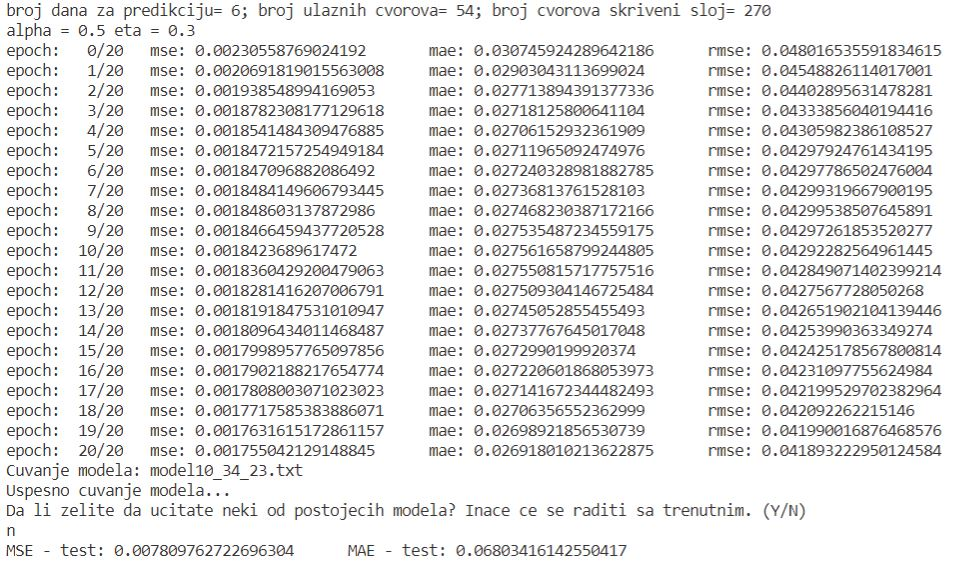
\includegraphics[scale=0.55]{output/output_example_program_10_34_23.JPG}
    \end{center}
\end{frame}

%--------------------------------------------------------
\begin{frame}{\small{Model \texttt{n = 54, m = 270, alpha = 0.5, eta = 0.3}}}
    \begin{figure}
    \centering
    \subfigure{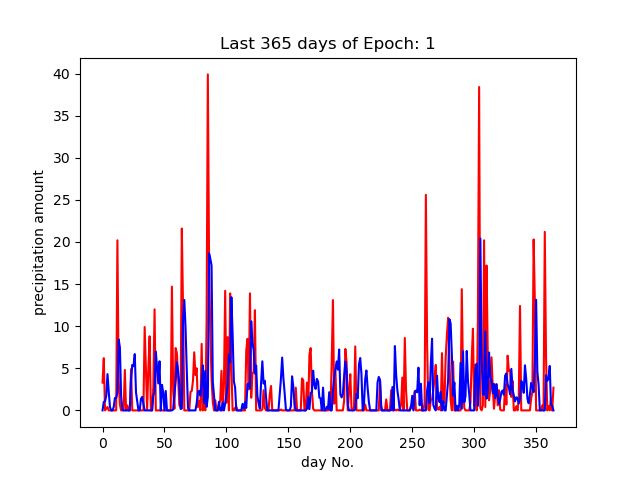
\includegraphics[width=0.45\linewidth]{plots/plot_epoch_1_time_10_34_23.png}} 
    \subfigure{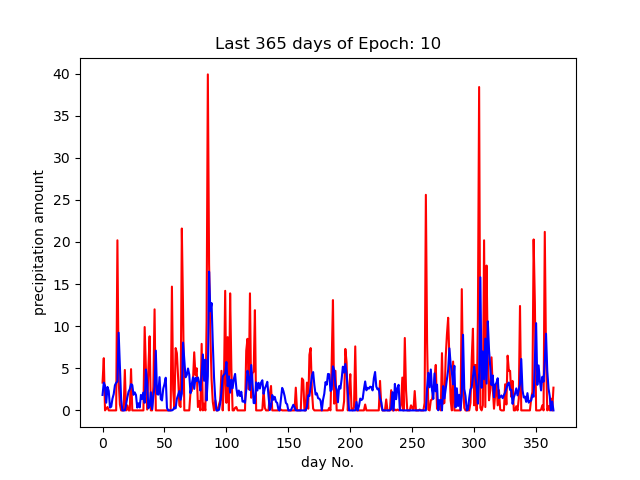
\includegraphics[width=0.45\linewidth]{plots/plot_epoch_10_time_10_34_23.png}} 
    \subfigure{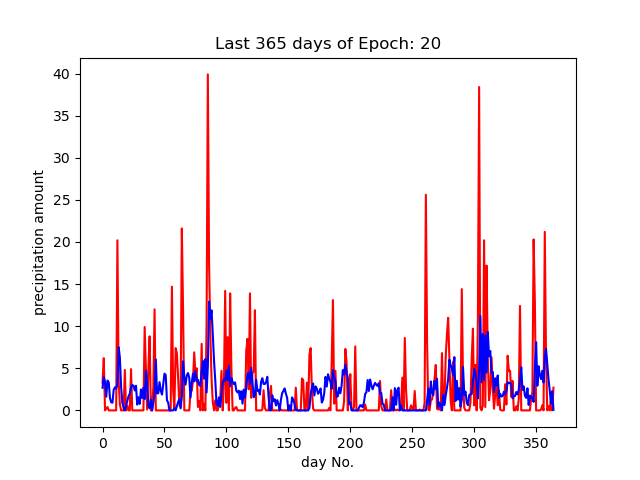
\includegraphics[width=0.45\linewidth]{plots/plot_epoch_20_time_10_34_23.png}}
    \subfigure{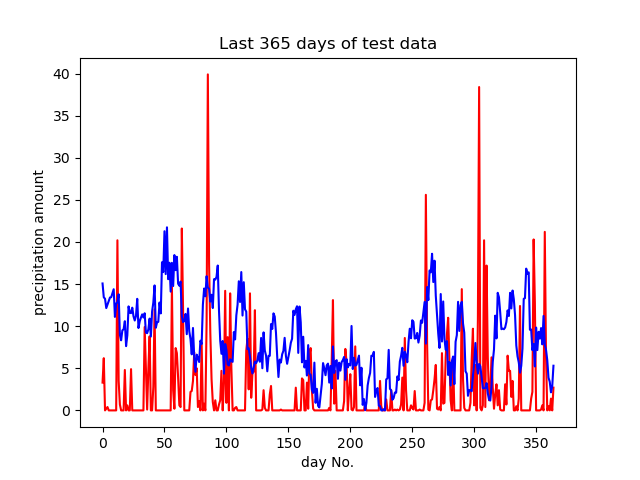
\includegraphics[width=0.45\linewidth]{plots/plot_test_model-model10_34_23-time_10_34_23.png}}
\end{figure}
\end{frame}


% ---------------------------------------------------------
\begin{frame}
    \begin{columns}
    
    \column{0.6\textwidth}
    \begin{figure}
        \centering
        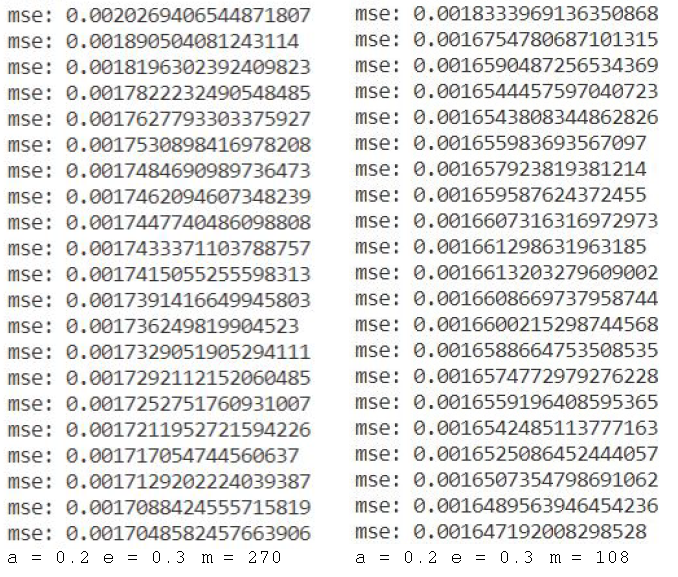
\includegraphics[scale=0.5]{presentation/poredjenje mse.png}
    \end{figure}
    
    \column{0.4\textwidth}
    \begin{figure}
        \begin{subfigure}{\textwidth}
            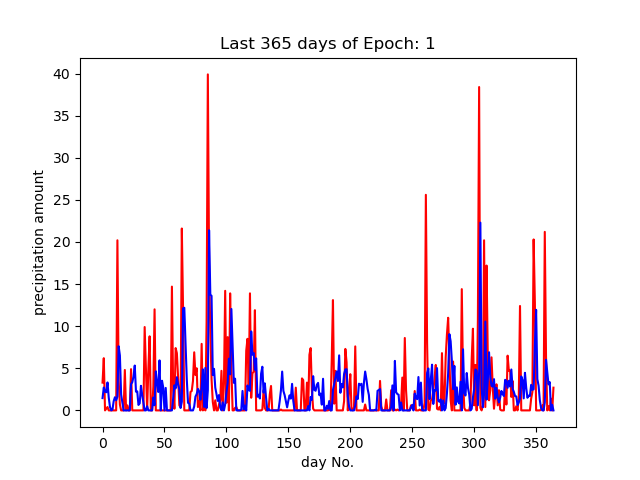
\includegraphics[width=\linewidth]{plots/plot_epoch_1_time_11_20_22.png}
            \caption*{m = 270, $\alpha$ = 0.2, $\eta$ = 0.3}
        \end{subfigure}
        \begin{subfigure}{\textwidth}
            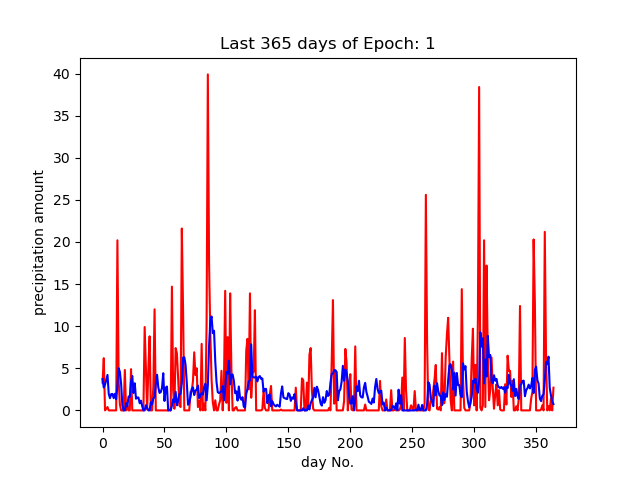
\includegraphics[width=\linewidth]{plots/plot_epoch_1_time_14_14_49.png}
            \caption*{m = 108, $\alpha$ = 0.2, $\eta$ = 0.3}
        \end{subfigure}
    \end{figure}
    \end{columns}

\end{frame}

% ==================================================== 2

% \begin{frame}{\small{Model \texttt{n = 54, m = 270, alpha = 0.2, eta = 0.3}}}
%     \begin{center}
%     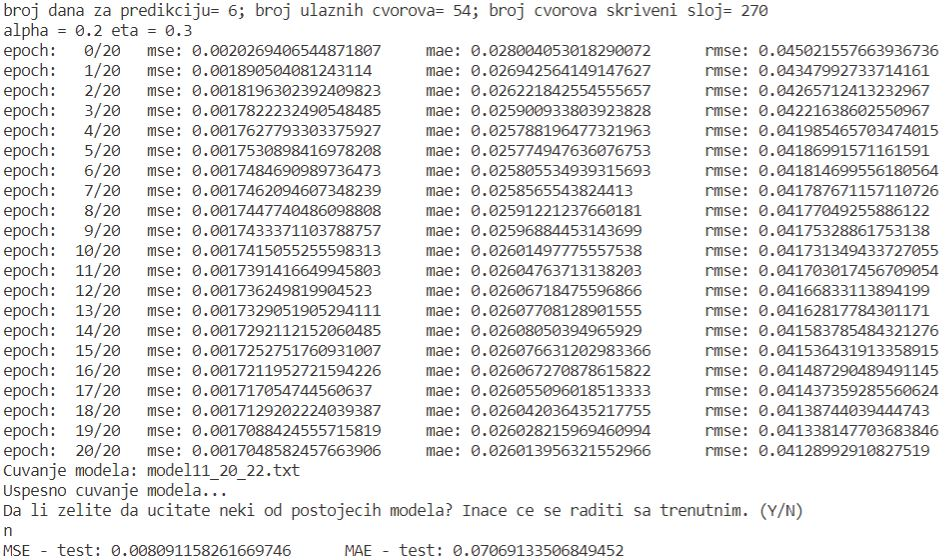
\includegraphics[scale=0.55]{output/output_example_program_11_20_22.JPG}
%     \end{center}
% \end{frame}

%--------------------------------------------------------
% \begin{frame}{\small{Model \texttt{n = 54, m = 270, alpha = 0.2, eta = 0.3}}}
%     \begin{figure}
%     \centering
%     \subfigure{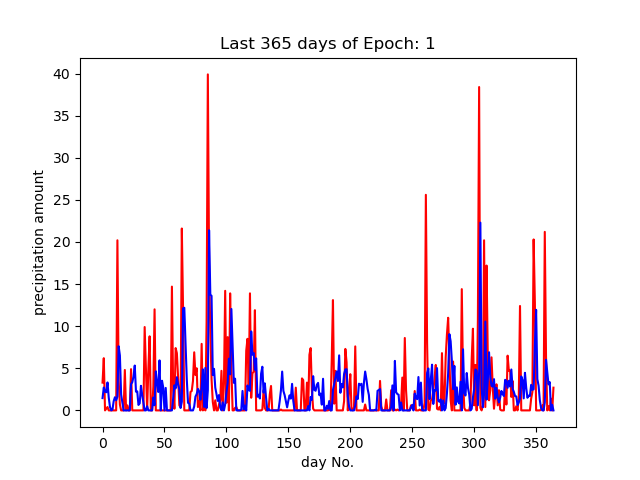
\includegraphics[width=0.45\textwidth]{plots/plot_epoch_1_time_11_20_22.png}} 
%     \subfigure{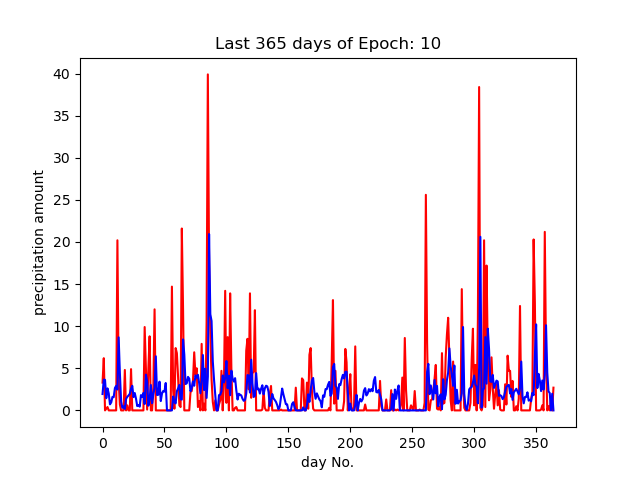
\includegraphics[width=0.45\textwidth]{plots/plot_epoch_10_time_11_20_22.png}} 
%     \subfigure{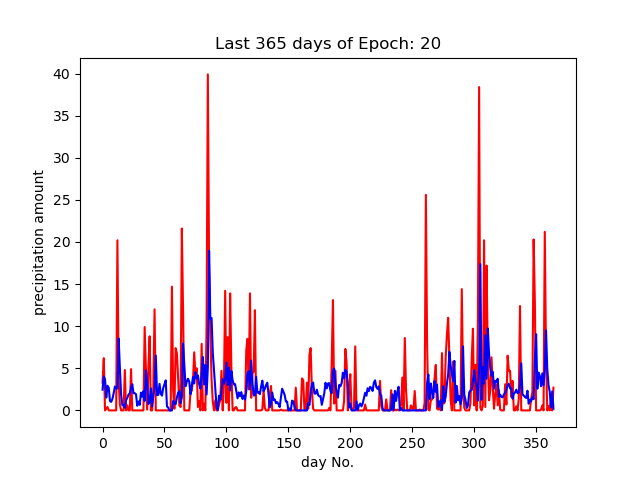
\includegraphics[width=0.45\textwidth]{plots/plot_epoch_20_time_11_20_22.png}}
%     \subfigure{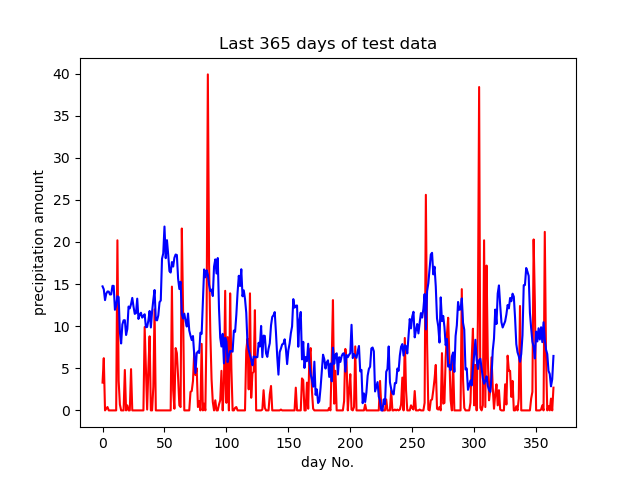
\includegraphics[width=0.45\textwidth]{plots/plot_test_model-model11_20_22-time_11_20_22.png}}
% \end{figure}
% \end{frame}

% ==================================================== dva modela uporedo, ovi kojima je prikazana prva epoha na slajdu za poredjenje mse

\begin{frame}{\small{m = 270, $\alpha$ = 0.2, $\eta$ = 0.3} \hspace{4cm} \small{m = 108, $\alpha$ = 0.2, $\eta$ = 0.3}}

    \begin{figure}
    % 1
        \begin{subfigure}{\textwidth}
            % \caption*{\small{m = 270, $\alpha$ = 0.2, $\eta$ = 0.3}}
            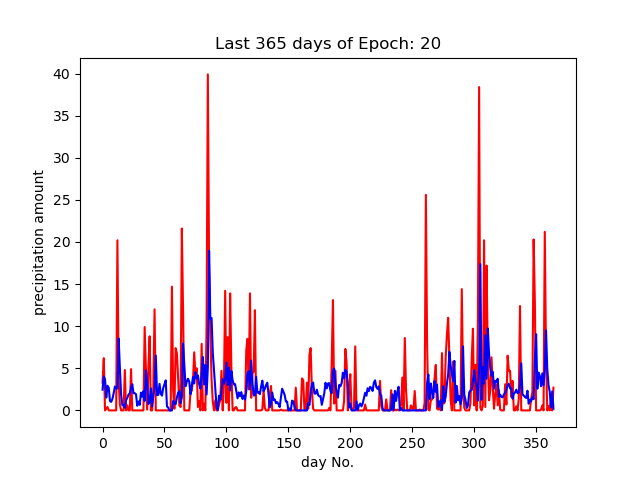
\includegraphics[width=0.45\linewidth]{plots/plot_epoch_20_time_11_20_22.png}
        \end{subfigure}
    % 2
        \begin{subfigure}{\textwidth}
            % \caption*{\small{m = 108, $\alpha$ = 0.2, $\eta$ = 0.3}}
            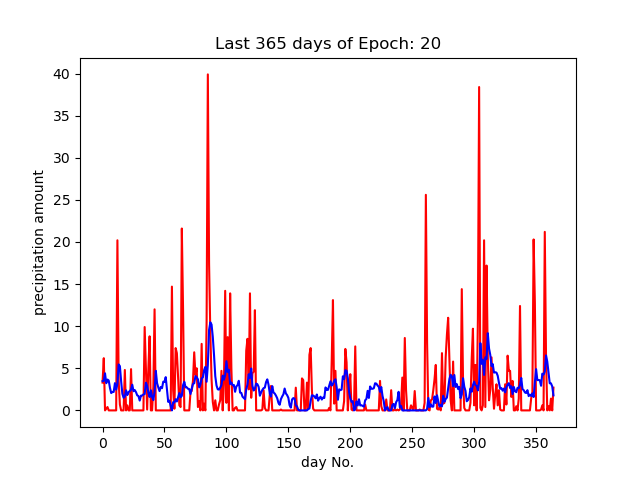
\includegraphics[width=0.45\linewidth]{plots/plot_epoch_20_time_14_14_49.png}
        \end{subfigure}
       
    % 1a
        \begin{subfigure}{\textwidth}
            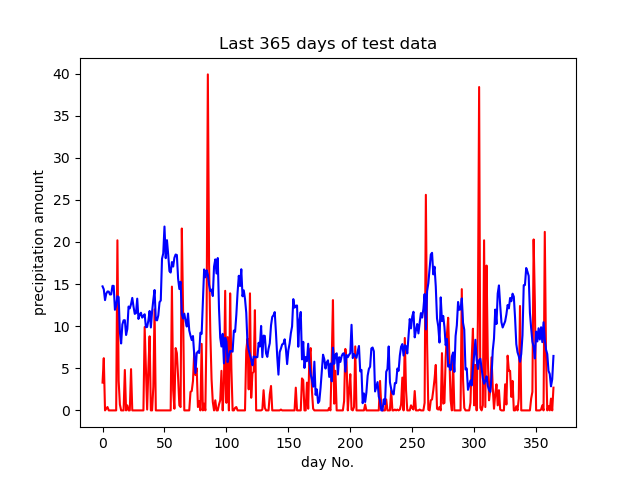
\includegraphics[width=0.45\linewidth]{plots/plot_test_model-model11_20_22-time_11_20_22.png}
        \end{subfigure}
    % 2a 
        \begin{subfigure}{\textwidth}
            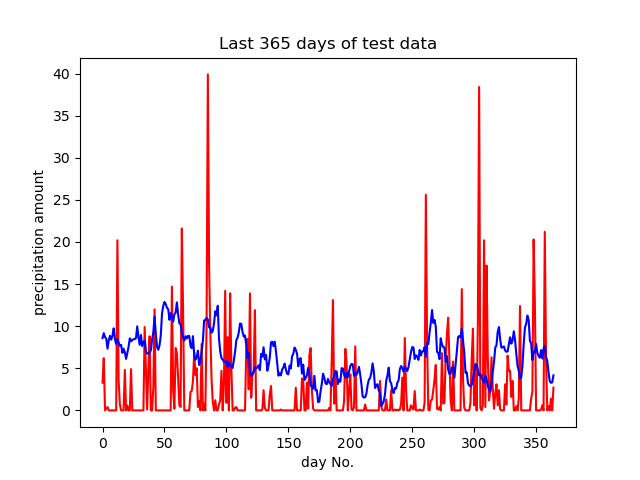
\includegraphics[width=0.45\linewidth]{plots/plot_test_model-model14_14_49-time_14_14_49.png}
        \end{subfigure}
    \end{figure}

\end{frame}


% ==================================================== 3

% \begin{frame}{\small{Model \texttt{n = 54, m = 108, alpha = 0.2, eta = 0.3}}}
%     \begin{center}
%     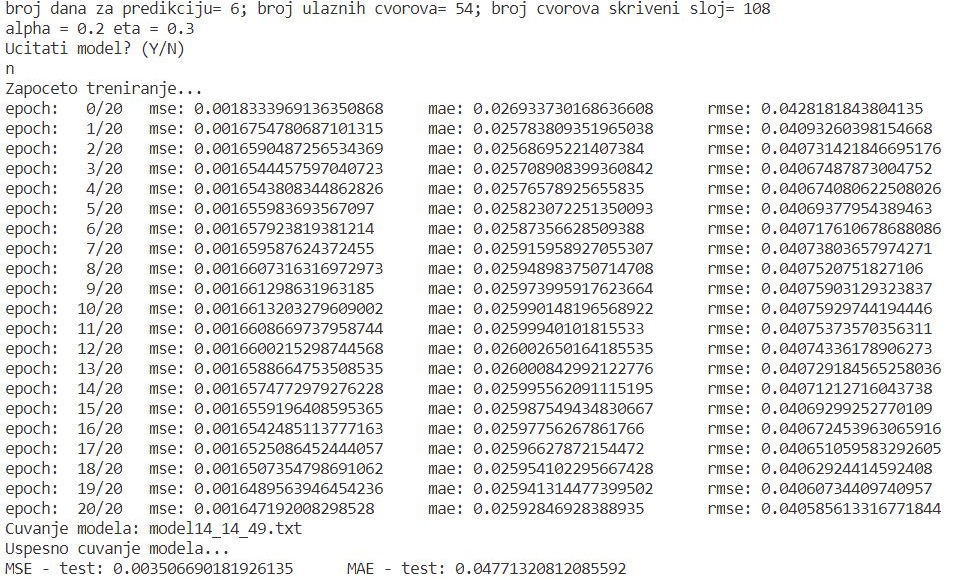
\includegraphics[scale=0.55]{output/output_example_program_14_14_49.JPG}
%     \end{center}
% \end{frame}

%--------------------------------------------------------
% \begin{frame}{\small{Model \texttt{n = 54, m = 108, alpha = 0.2, eta = 0.3}}}
%     \begin{figure}
%     \centering
%     \subfigure{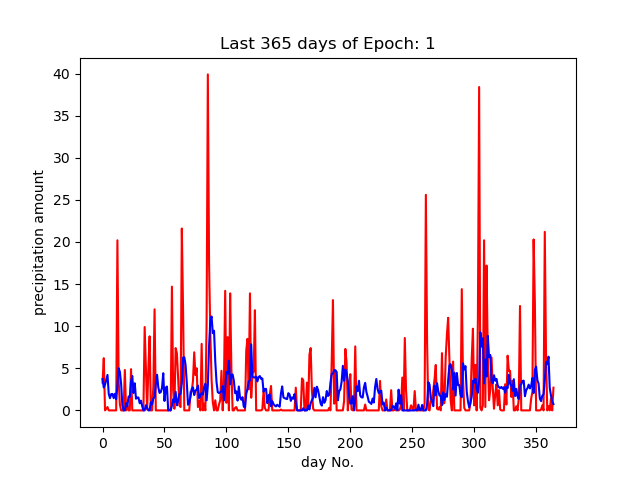
\includegraphics[width=0.45\textwidth]{plots/plot_epoch_1_time_14_14_49.png}} 
%     \subfigure{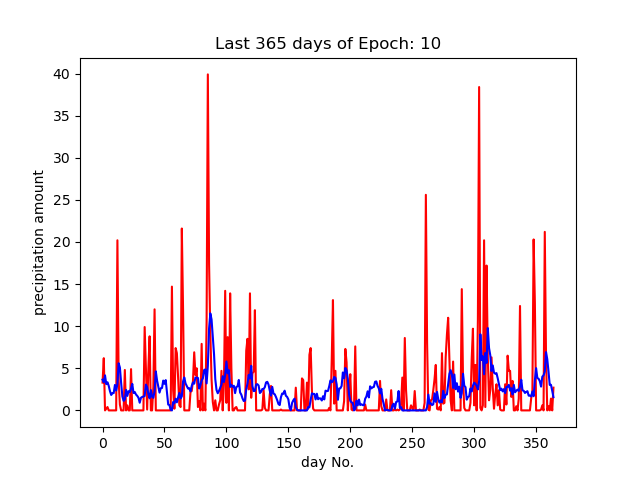
\includegraphics[width=0.45\textwidth]{plots/plot_epoch_10_time_14_14_49.png}} 
%     \subfigure{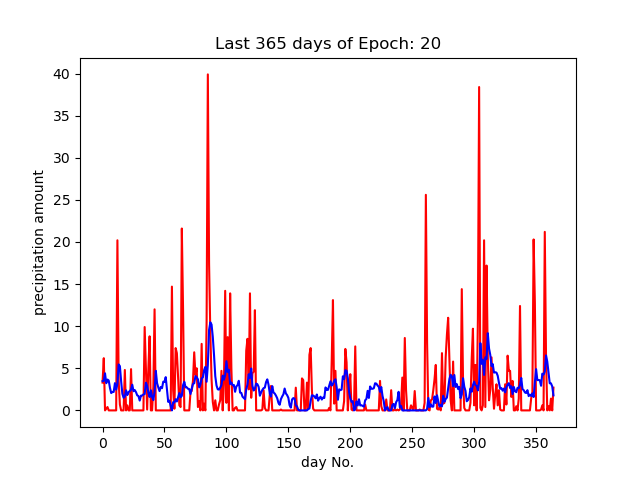
\includegraphics[width=0.45\textwidth]{plots/plot_epoch_20_time_14_14_49.png}}
%     \subfigure{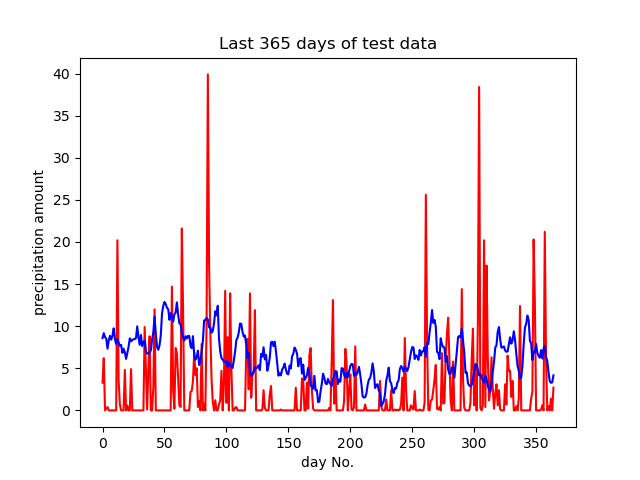
\includegraphics[width=0.45\textwidth]{plots/plot_test_model-model14_14_49-time_14_14_49.png}}
% \end{figure}
% \end{frame}

% ==================================================== 4

% \begin{frame}{\small{{Model \texttt{n = 54, m = 108, alpha = 0.9, eta = 0.5}}}}
%     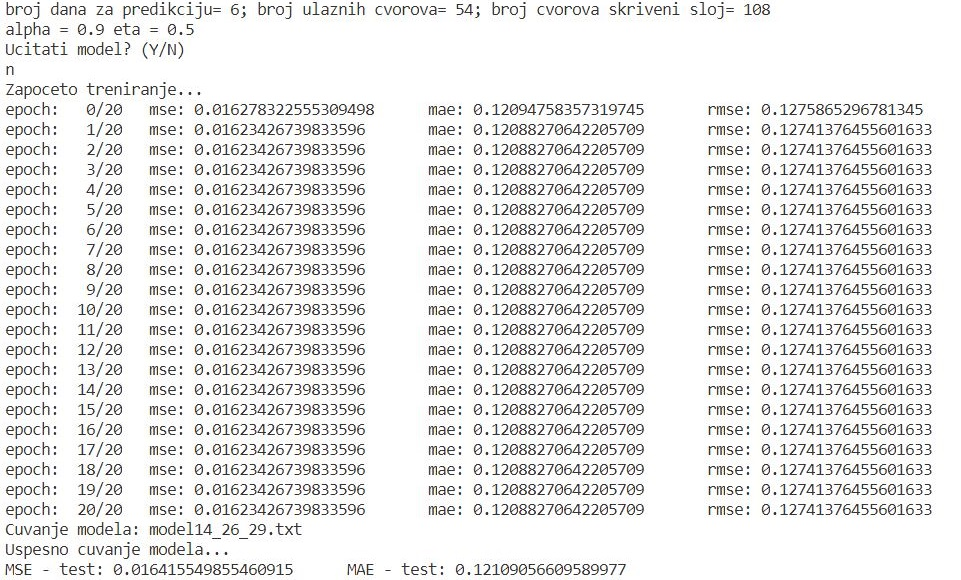
\includegraphics[scale=0.55]{output/output_example_program_14_26_29.JPG}
% \end{frame}

%--------------------------------------------------------
% Napomeni da za vrednost alpha = 0.9 ode u minimum i ne moze da se izvuce iz njega.

% \begin{frame}{\small{{Model \texttt{n = 54, m = 108, alpha = 0.9, eta = 0.5}}}}
%     \begin{figure}
%     \centering
%     \subfigure{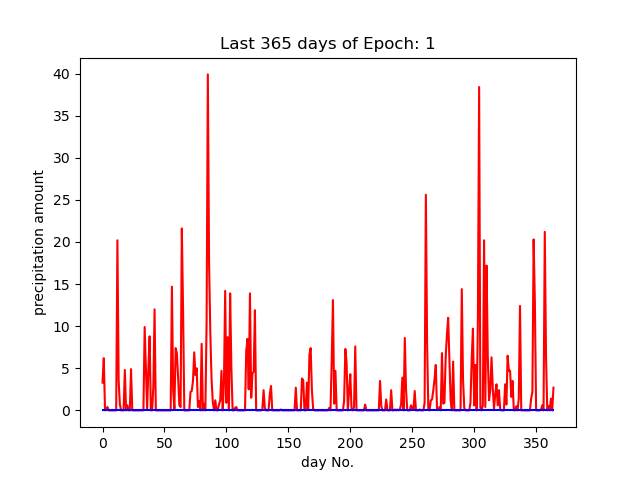
\includegraphics[width=0.45\textwidth]{plots/plot_epoch_1_time_14_26_29.png}} 
%     \subfigure{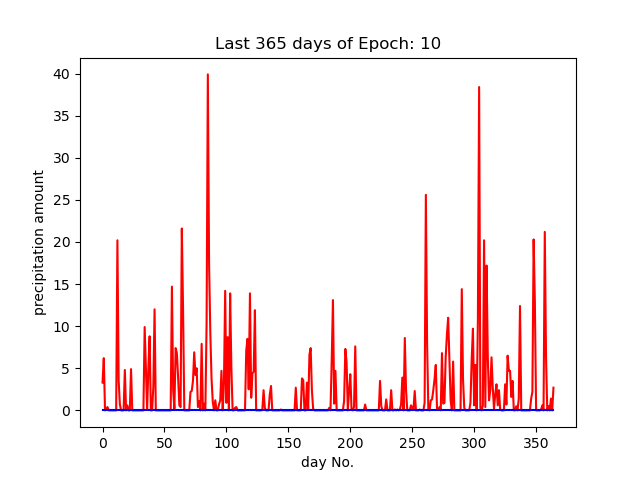
\includegraphics[width=0.45\textwidth]{plots/plot_epoch_10_time_14_26_29.png}} 
%     \subfigure{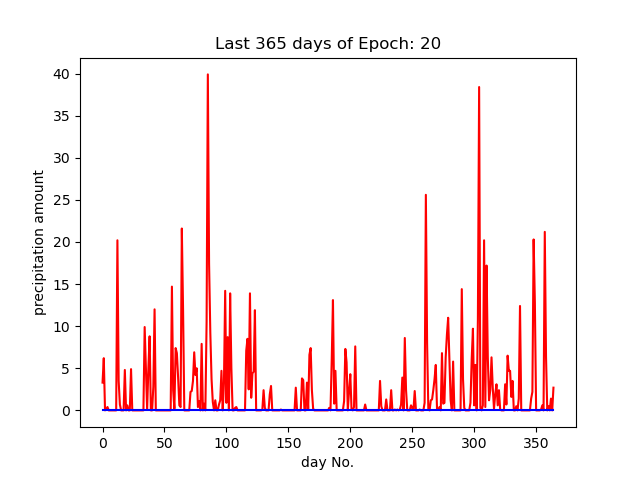
\includegraphics[width=0.45\textwidth]{plots/plot_epoch_20_time_14_26_29.png}}
%     \subfigure{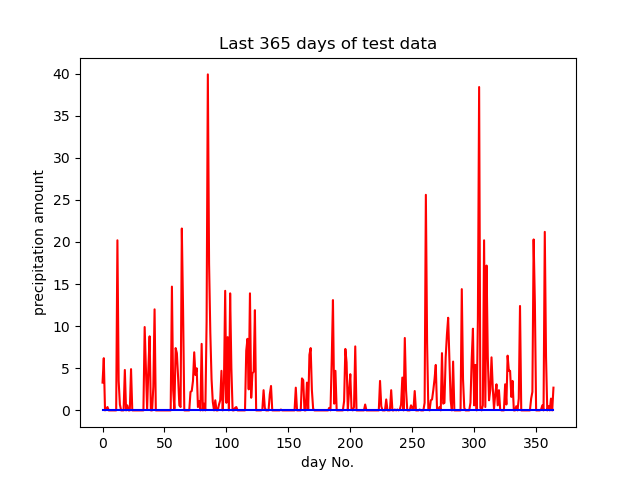
\includegraphics[width=0.45\textwidth]{plots/plot_test_model-model14_26_29-time_14_26_29.png}}
% \end{figure}
% \end{frame}

% ==================================================== 5

% \begin{frame}{\small{{Model \texttt{n = 54, m = 216, alpha = 0.2, eta = 0.3}}}}
%     \begin{center}
%     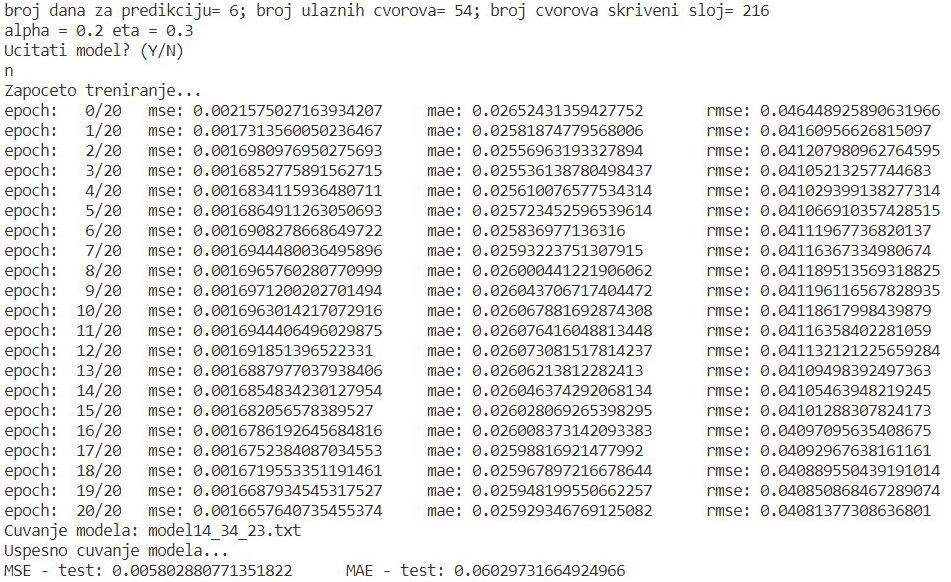
\includegraphics[scale=0.55]{output/output_example_program_14_34_23.JPG}
%     \end{center}
% \end{frame}

%--------------------------------------------------------
%  mislim da ovaj ne mora da se prikaze
% \begin{frame}{\small{{Model \texttt{n = 54, m = 216, alpha = 0.2, eta = 0.3}}}}
%     \begin{figure}
%     \centering
%     \subfigure{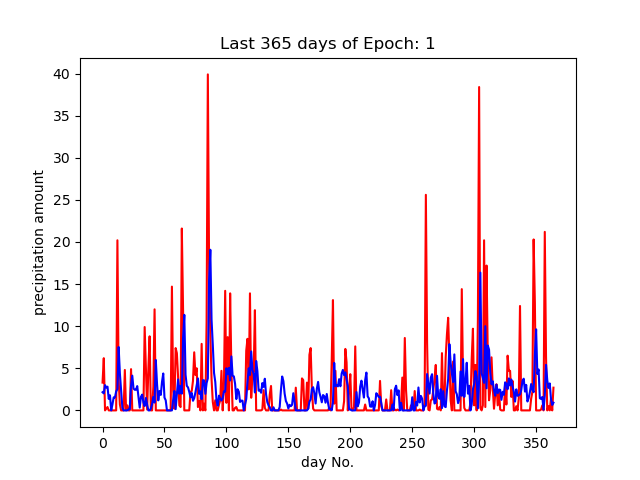
\includegraphics[width=0.45\textwidth]{plots/plot_epoch_1_time_14_34_23.png}} 
%     \subfigure{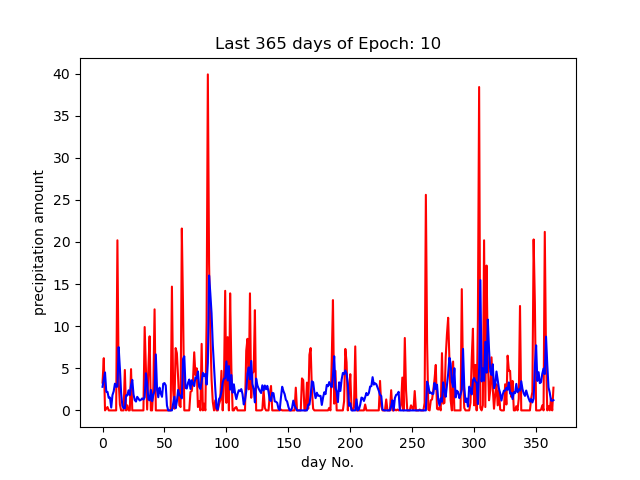
\includegraphics[width=0.45\textwidth]{plots/plot_epoch_10_time_14_34_23.png}} 
%     \subfigure{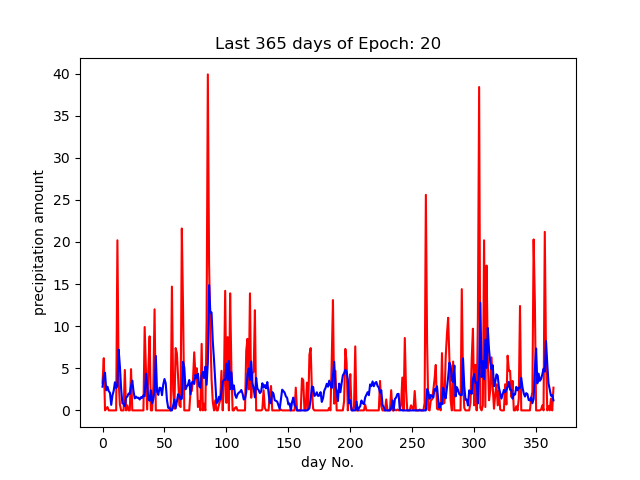
\includegraphics[width=0.45\textwidth]{plots/plot_epoch_20_time_14_34_23.png}}
%     \subfigure{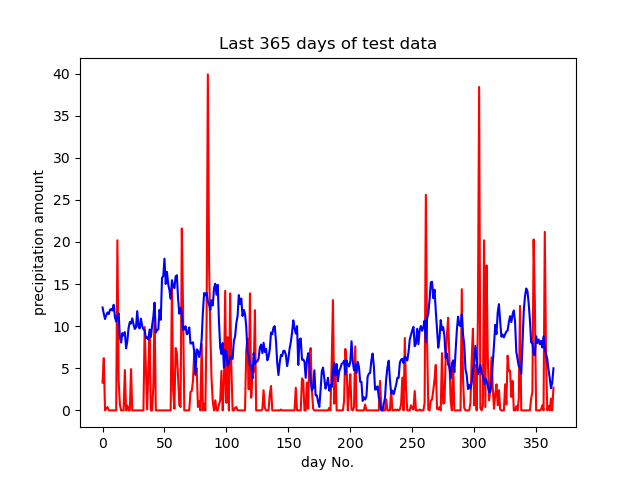
\includegraphics[width=0.45\textwidth]{plots/plot_test_model-model14_34_23-time_14_34_23.png}}
% \end{figure}
% \end{frame}

\section{Zaključak}

%--------------------------------------------------------
% \appendix

\begin{frame}{References}
    \nocite{*} % Display all references regardless of if they were cited
	\bibliography{seminarski.bib}
	\bibliographystyle{plain}
\end{frame}

\end{document}